\section{Tipografia}
\begin{frame}
\frametitle{Escribas}
\begin{figure}[htbp]
\centering
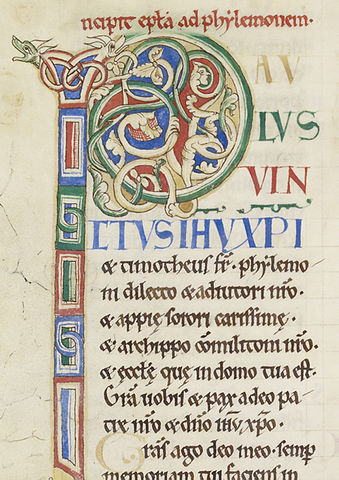
\includegraphics[width=0.35\textwidth,height=0.75\textheight,keepaspectratio]{figures/rochester_bible.jpg}
\caption{Primeira página da epístola de Paulo a Filêmon na Bíblia de Rochester (século 12).}
\label{fig-rochester_bible}
\end{figure}
\end{frame}
\note{
A preocupação com a estética dos textos é antiga.
Esta figura mostra um exemplos de escrita gótica utilizada pelos escribas nas cópias manuais que faziam 
do texto da bíblia.
É evidente a preocupação com a ornamentação e a elaboração de um visual rebuscado.

Quando Gutenberg criou os primeiros tipos móveis, para realizar cópias da bíblia, buscou ainda manter 
a escrita gótica.
}


\begin{frame}
\frametitle{Gutenberg}
\begin{figure}[htbp]
\begin{minipage}[t]{0.47\textwidth}
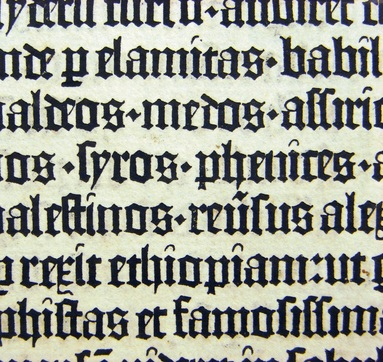
\includegraphics[width=0.8\linewidth,height=0.5\textheight,keepaspectratio]{figures/gutenberg.jpg}
\subcaption{Bíblia de Gutenberg.}
\end{minipage}
\hfill
\begin{minipage}[t]{0.47\textwidth}
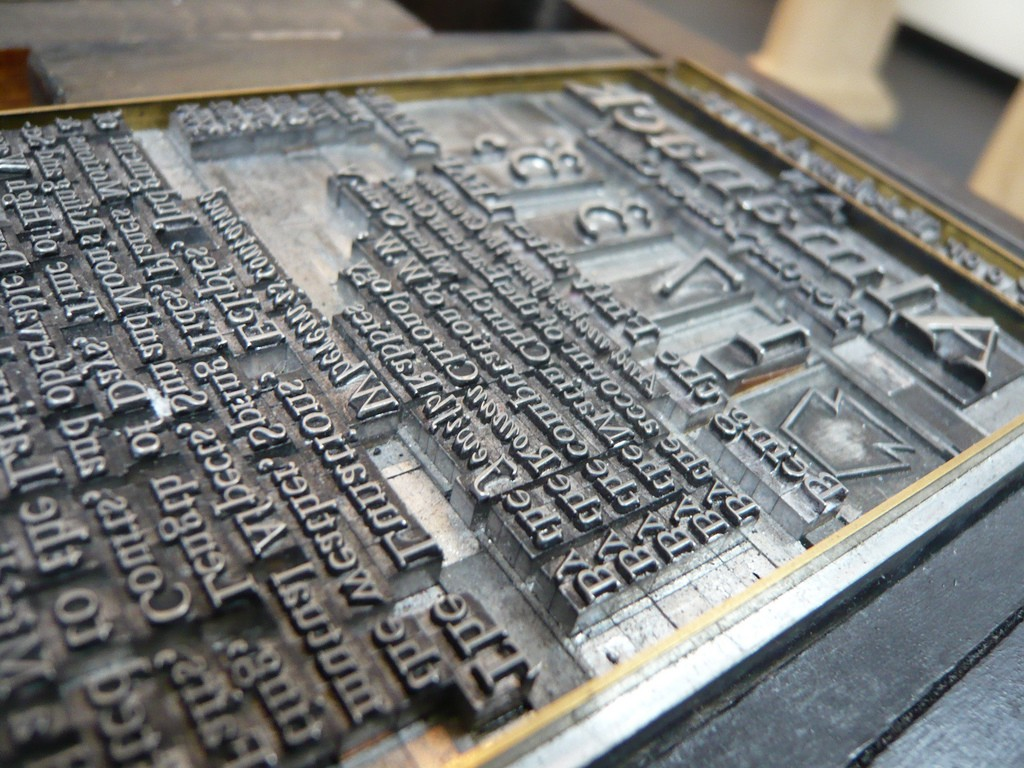
\includegraphics[width=\linewidth,height=0.5\textheight,keepaspectratio]{figures/mov-type.jpg}
\subcaption{Tipos móveis.}
\end{minipage}
\caption{Tipografia moderna.}
\end{figure}
\end{frame}

\begin{frame}[allowframebreaks]
\frametitle{A nova tipografia - Jan Tschichold, 1928}
\begin{figure}[htbp]
\centering
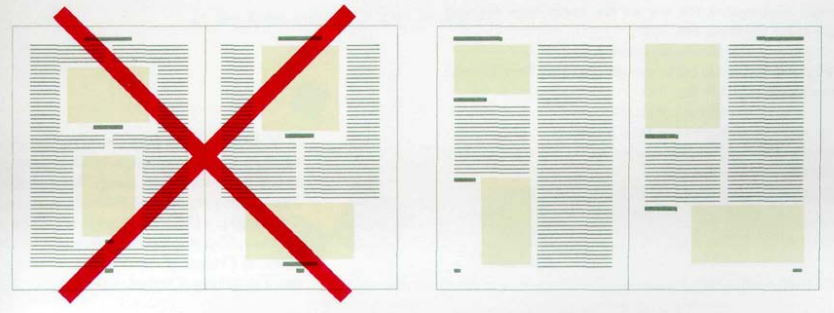
\includegraphics[width=\textwidth,height=0.5\textheight,keepaspectratio]{figures/jan-tschichold.png}
\caption{Comparação entre layouts.}
\label{fig-jan-tschichold}
\end{figure}

\begin{quote}
Trabalhar um texto de acordo com esses princípios geralmente resultará em um
ritmo diferente daquele da tipografia simétrica anterior. A assimetria é a
expressão rítmica do design funcional. Além de ser mais lógica, a assimetria
tem a vantagem de que sua aparência completa é muito mais eficaz opticamente do
que a simetria.
%Working through a text according to these principles will usually result in a
%rhythm different from that of former symmetrical typography. Asymmetry is the
%rhythmic expression of functional design. In addition to being more logical,
%asymmetry has the advantage that its complete appearance is far more optically
%effective than symmetry.
\end{quote}

\begin{quote} 
Daí o predomínio da assimetria na Nova Tipografia. Não menos importante, a
vivacidade da assimetria é também uma expressão de nosso próprio movimento e
este da vida moderna; é um símbolo das formas mutáveis da vida em geral, quando
o movimento assimétrico na tipografia toma o lugar do repouso simétrico. Este
movimento não deve, entretanto, degenerar em agitação ou caos. A busca pela
ordem também pode e deve ser expressa de forma assimétrica. É a única maneira
de tornar possível uma ordem melhor e mais natural, em oposição à forma
simétrica, que não extrai suas leis de dentro, mas de fora. 
%Hence the predominance of asymmetry in the New Typography. Not least, the
%liveliness of asymmetry is also an expression of our own movement and that of
%modern life; it is a symbol of the changing forms of life in general when
%asymmetrical movement in typography takes the place of symmetrical repose. This
%movement must not, however, degenerate into unrest or chaos. A striving for
%order can, and must, also be expressed in asymmetrical form. It is the only way
%to make a better, more natural order possible, as opposed to symmetrical form,
%which does not draw its laws from within itself but from outside.
\end{quote}

% https://readings.design/PDF/ThePrinciplesoftheNewTypography.pdf
% https://medium.com/@digitalonetwo/the-new-typography-excerpt-c2a3c1325f23
% https://www.fontfabric.com/blog/gutenberg-first-typeface-original-bible-typography-used/
\end{frame}


\begin{frame}
\frametitle{Recursos tipográficos}
O \TeX{} utiliza recursos tipográficos para melhorar a leitura e
a aparência (ou agradabilidade) dos textos.

Alguns deles são:
\begin{itemize}
  \item Ligadura
  \item Kerning
  \item Hifenização
  \item Quebra de linhas
  \item Justificação
  \item Quebra de parágrafos
  \item Controle de órfãos 
\end{itemize}
\end{frame}

\begin{frame}
\frametitle{\TeX{}}
\framesubtitle{Ligadura}

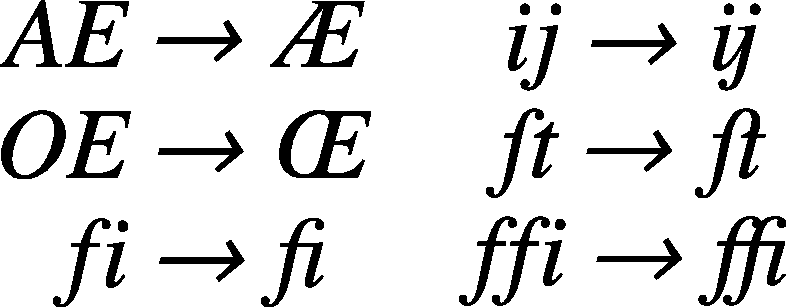
\includegraphics[width=0.35\linewidth]{figures/ligatures.pdf} \hspace{4em}
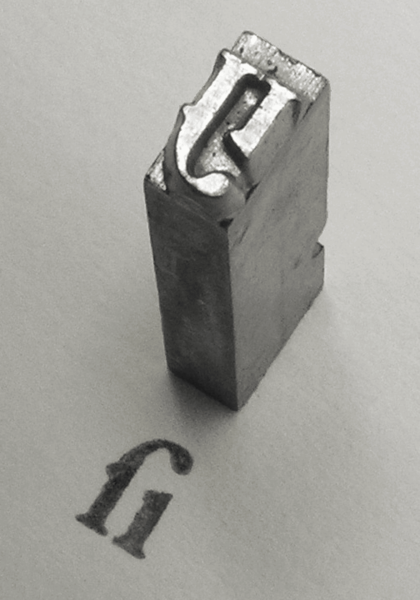
\includegraphics[width=0.15\linewidth]{figures/ligatures_fi.png}

\vspace{2ex}
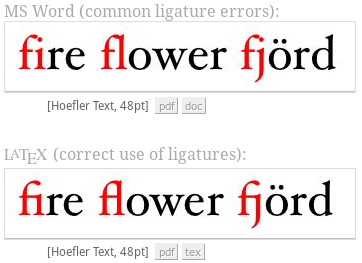
\includegraphics[width=0.3\linewidth]{figures/fire_ligatures.png}
\end{frame}


\begin{frame}
\frametitle{\TeX{}}
\framesubtitle{Kerning}
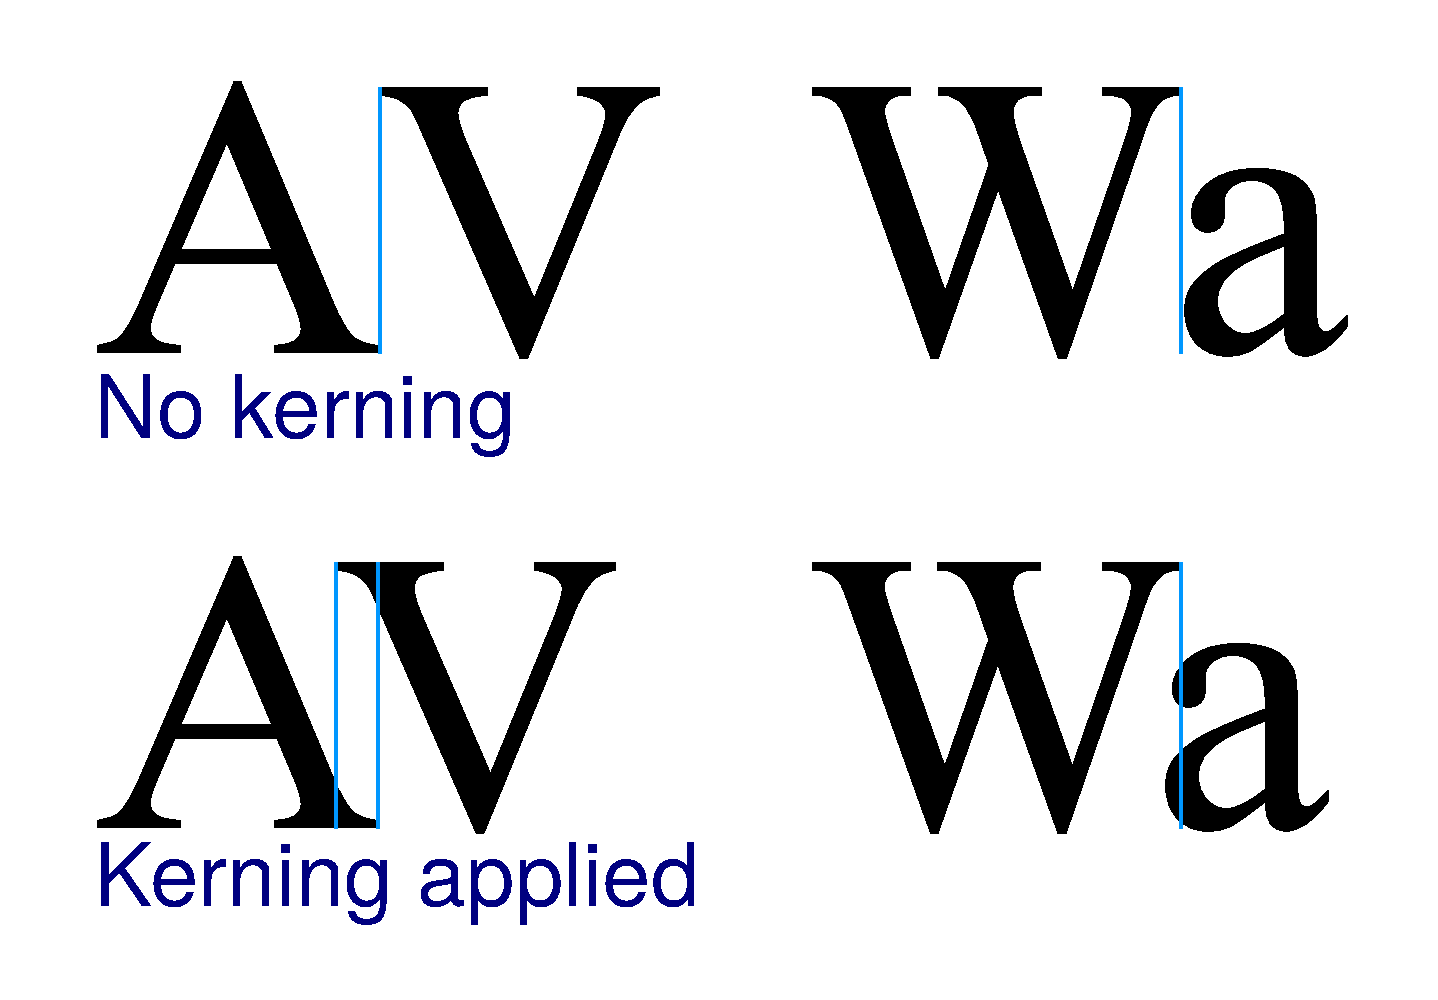
\includegraphics[width=0.3\linewidth]{figures/kerning.pdf}

\vspace{2ex}
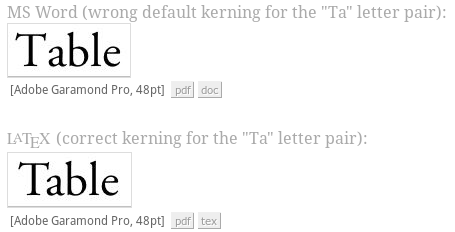
\includegraphics[width=0.4\linewidth]{figures/table_kerning.png}

\footnotesize{(Wikipedia, \url{http://nitens.org/taraborelli/latex})}
\end{frame}


\begin{frame}
\frametitle{Sugestão de leitura}

\fullcite{huyett2014}
\vspace{2ex}

\fullcite{schannel2019}
\vspace{2ex}

\fullcite{stephen2018}
\vspace{2ex}

\fullcite{satori2019}
\vspace{2ex}

\fullcite{history2018}

\end{frame}
